% !TEX root = ./Report.tex

\documentclass[a4paper,11pt]{article}
\usepackage[utf8]{inputenc}
\usepackage{graphicx}
\usepackage{hyperref}
\usepackage{amsmath}
\usepackage{amsfonts} 
\usepackage{booktabs}
\usepackage{caption}
\usepackage{float}

% Dati studente
\title{\textbf{Homework 2: IMAGE CLASSIFICATION}}
\author{Sara Cristina Basco (Student Number: 2256687)}
\date{\today}

\begin{document}

\maketitle
\section{Introduction}
The objective of this project is to develop a robust computer vision system for autonomous agents operating in the RoboCup environment. The task consists of learning a mapping function $f(I) \rightarrow \{c, (x,y)\}$, which predicts the semantic class $c$ and the normalized object position $(x,y)$ given a raw RGB input image $I$.

\paragraph{Experimental Setup}
This work evaluates the visual perception pipeline on a dataset characterizing the typical unstructured environment of robotic soccer, characterized by variable lighting and occlusions.

\paragraph{Dataset Description}
The experimental data is derived from the SPQR Dataset. The problem is decomposed into two sub-tasks with varying input specifications:

\begin{itemize}
    \item \textbf{Task 1: Classification.} The objective is to assign a discrete label $c \in \mathcal{C}$ to the image, where $\mathcal{C} = \{\text{Ball, Robot, GoalPost, ...}\}$. The input images are resized to $64 \times 64$ pixels to prioritize semantic feature extraction speed.
    
    \item \textbf{Task 2: Regression (Localization).} The objective is to predict the continuous vector $v = (x, y) \in [0, 1]^2$ representing the object's center. The input images are processed at $128 \times 128$ pixels to maintain sufficient spatial resolution for accurate localization.
\end{itemize}

\section{Data Loading and Preprocessing}

To efficiently manage the data ingestion pipeline, a custom dataset class named \texttt{SoccerDataset}, inheriting from \texttt{torch.utils.data.Dataset}, was implemented. Unlike standard directory-based data loaders, this implementation parses a CSV annotation file containing image filenames, object class labels, and bounding box coordinates.

The dataset class is designed to operate in two distinct modes, controlled by a \texttt{task} parameter, in order to support the specific requirements of the two neural network architectures employed in this work.

\paragraph{Mode A: Classification}
The primary objective of this mode is semantic object recognition. For each sample, the \texttt{\_\_getitem\_\_} method performs the following operations:
\begin{itemize}
    \item \textbf{Image loading}: the RGB image file is read from disk.
    \item \textbf{Resizing}: the image is downsampled to a resolution of $64 \times 64$ pixels. This resolution was empirically found to be sufficient for capturing the macro-level visual features required to distinguish between classes (e.g., the spherical shape of the ball versus the vertical structure of the goalpost), while significantly reducing computational cost.
    \item \textbf{Label encoding}: the categorical class label (e.g., \texttt{robot}) is mapped to a discrete integer index $y \in \{0, 1, \dots, 4\}$.
    \item \textbf{Transformation}: pixel values are converted into a \texttt{FloatTensor} and normalized to the range $[0, 1]$.
\end{itemize}

\paragraph{Mode B: Regression}
The objective of this mode is spatial object localization. In this case, the preprocessing pipeline differs in two key aspects:
\begin{itemize}
    \item \textbf{High-resolution input}: images are resized to $128 \times 128$ pixels in order to preserve finer spatial details that are necessary for accurate coordinate regression.
    \item \textbf{Target normalization}: the bounding box coordinates provided in the CSV file $(x_{\min}, y_{\min}, x_{\max}, y_{\max})$ are converted into the relative center of the object $(c_x, c_y)$. The coordinates are normalized with respect to the image width $W$ and height $H$ as follows:
\end{itemize}

\begin{equation}
\hat{x} = \frac{(x_{\min} + x_{\max}) / 2}{W},
\qquad
\hat{y} = \frac{(y_{\min} + y_{\max}) / 2}{H}
\end{equation}

This normalization ensures that the regression targets lie within the bounded interval $[0, 1]$, thereby decoupling the model from the absolute image resolution and contributing to more stable gradient-based optimization during training.

This flexible dataset design enables the use of a single data source for training two separate models with different input and output requirements, while ensuring data consistency and promoting code reusability.

\section{Neural Architectures}

As a first approach to the perception problem, this work adopts two relatively simple Convolutional Neural Network (CNN) architectures implemented using the \texttt{torch.nn.Module} interface. The goal is to establish clear and interpretable baseline models for object classification and spatial localization, rather than optimizing for architectural complexity.

The classification model follows a standard feature extraction paradigm, while the regression model introduces a conditional design that allows spatial predictions to be influenced by semantic information through a late fusion strategy.

\subsection{Classification Model (ClassificationCNN)}

The objective of the classification network is to map an input image tensor
$X \in \mathbb{R}^{3 \times 64 \times 64}$ to a probability distribution over $K = 5$ object classes.
The architecture consists of two main components.

\begin{itemize}
    \item \textbf{Feature extractor:} a sequence of three convolutional blocks. Each block is composed of a \texttt{Conv2d} layer with increasing channel depth (16, 32, and 64), followed by a ReLU activation function and a $2 \times 2$ max-pooling operation. This design allows the network to progressively extract higher-level visual features while reducing the spatial resolution.

    \item \textbf{Classifier head:} the resulting feature map is flattened into a one-dimensional vector and processed by fully connected layers, producing a vector of logits $z \in \mathbb{R}^{5}$ corresponding to the object classes.
\end{itemize}

This architecture provides a simple and effective baseline for semantic object recognition on low-resolution inputs.

\subsection{Regression Model (RegressionCNN)}

The regression task is more challenging, as the definition of the object center
depends on the object category (e.g., the center of a ball versus the center of a
robot). To address this issue, a conditional CNN architecture based on a late
fusion strategy is employed.

The model takes as input an RGB image $I$ and the corresponding object class
label $c$.

\paragraph{Visual stream.}
The input image is resized to $128 \times 128$ pixels and processed by a CNN
backbone with increased depth, producing a visual feature vector
$v_{\text{img}}$.

\paragraph{Semantic stream.}
The discrete class label $c$ is encoded as a one-hot vector and projected through
a linear layer to obtain a low-dimensional semantic embedding
$v_{\text{sem}}$.

\paragraph{Late fusion.}
The visual and semantic feature vectors are concatenated to form a fused
representation
$v_{\text{fused}} = \mathrm{concat}(v_{\text{img}}, v_{\text{sem}})$,
which allows the regression network to condition spatial predictions on semantic
information.

\paragraph{Regression head.}
The fused feature vector is processed by fully connected layers to output the
predicted normalized object center
$\hat{\mathbf{y}} = (\hat{x}, \hat{y}) \in [0,1]^2$.

\section{Training Strategy}

All experiments were implemented in PyTorch and executed in a containerized
Docker environment. Due to computational constraints, training was performed
entirely on CPU. Training hyperparameters were therefore selected to balance
convergence speed and model performance.

\subsection{Loss Functions}

Two different loss functions were used to reflect the nature of the learning
tasks.

\textbf{Task 1: Cross Entropy Loss (Classification)}
For the classification task, the Cross Entropy loss was adopted to measure the
discrepancy between predicted class probabilities and ground-truth labels.


\textbf{Task 2: Mean Squared Error (Regression)}
For the regression task, the goal is to minimize the distance between the
predicted object center $\hat{\mathbf{y}} = (\hat{x}, \hat{y})$ and the
corresponding ground-truth normalized coordinates $\mathbf{y}$. 

MSE is well suited for localization tasks, as it strongly penalizes large
prediction errors and encourages rapid correction of inaccurate spatial
estimates.

\subsection{Optimization}

Model parameters were optimized using the Adam optimizer. Adam was chosen for
its adaptive learning rates and momentum-based updates, which promote faster
and more stable convergence compared to standard stochastic gradient descent,
especially under limited computational resources.

\subsection{Hyperparameters}

The training hyperparameters for both models are summarized in
Table~\ref{tab:hyperparams}. The regression model uses a higher input resolution
and more training epochs to account for the increased complexity of predicting
precise spatial coordinates.

\begin{table}[H]
\centering
\begin{tabular}{|l|c|c|}
\hline
\textbf{Parameter} & \textbf{Classification} & \textbf{Regression} \\
\hline
Optimizer & Adam & Adam \\
Learning rate & 0.001 & 0.001 \\
Batch size & 32 & 32 \\
Epochs & 5 & 10 \\
Image size & $64 \times 64$ & $128 \times 128$ \\
\hline
\end{tabular}
\caption{Training hyperparameters for the classification and regression models.}
\label{tab:hyperparams}
\end{table}

\section{Experimental Results}

The proposed models were evaluated on a held-out test set using both quantitative
metrics and qualitative visual inspection. All experiments were executed in a
CPU-based Docker environment, highlighting the lightweight nature of the
architectures.

\subsection{Quantitative Analysis}

Table~\ref{tab:results} reports the final metrics obtained after training.

\begin{table}[h]
\centering
\begin{tabular}{|l|c|c|}
\hline
\textbf{Metric} & \textbf{Classification} & \textbf{Regression} \\
\hline
Epochs & 5 & 10 \\
Final loss & 0.5147 (Cross Entropy) & 0.0383 (MSE) \\
Accuracy / performance & \textbf{83.02\%} & MSE: 0.0383 \\
Training time & 1 min 7 s & 5 min 42 s \\
\hline
\end{tabular}
\caption{Quantitative results on the test set.}
\label{tab:results}
\end{table}

The classification model achieved an accuracy of 83.02\% after only five epochs,
with a final loss of 0.5147, indicating stable and effective learning of the five
object categories. The regression task required longer training due to its
higher complexity, but achieved a low Mean Squared Error of 0.0383 on normalized
coordinates, demonstrating accurate object center localization.

\subsection{Qualitative Evaluation and Error Analysis}
To provide a comprehensive assessment, we analyze both successful predictions and failure cases. Figure \ref{fig:comparison} compares two distinct scenarios regarding the interaction between classification and regression.

\begin{figure}[H]
    \centering
    % PRIMA IMMAGINE (SUCCESSO)
    \begin{minipage}{0.48\textwidth}
        \centering
        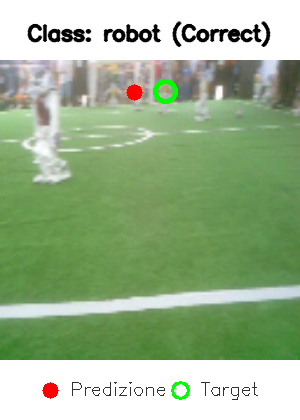
\includegraphics[width=\linewidth]{prediction_success.png} 
        \caption*{\textbf{(a) Success Case}}
    \end{minipage}
    \hfill
    % SECONDA IMMAGINE (ERRORE)
    \begin{minipage}{0.48\textwidth}
        \centering
        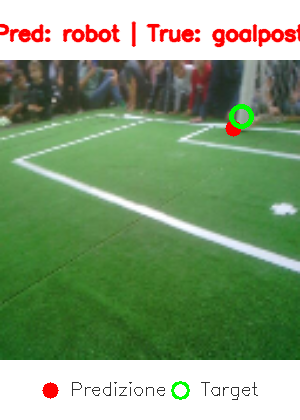
\includegraphics[width=\linewidth]{prediction_error.png}
        \caption*{\textbf{(b) Failure Case}}
    \end{minipage}
    
    \caption{\textbf{Qualitative Comparison.} 
    \textbf{(a)} The model correctly identifies the \textit{Robot} and the regression (Red Dot) precisely overlaps with the Ground Truth (Green Circle).
    \textbf{(b)} An example of misclassification: the model predicts \textit{Robot} instead of \textit{Goalpost} (indicated by the red text). Interestingly, the regression still attempts to localize the object, but the semantic mismatch leads to a slight localization offset. This highlights the dependency of the Late Fusion module on accurate classification.}
    \label{fig:comparison}
\end{figure}

As shown in Case (a), when the semantic stream is correct, the localization is highly accurate. Case (b) demonstrates a limitation: visual ambiguity (e.g., white lines vs. white robot parts) can lead to classification errors. However, the system remains robust enough to identify the region of interest, even if the label is incorrect.


\end{document}

